%----------------------------------------------------------------
%
%  File    :  thesis.tex
%
%  Authors :  Keith Andrews, IICM, TU Graz, Austria
%             Manuel Koschuch, FH Campus Wien, Austria
%			  Sebastian Ukleja, FH Campus Wien, Austria
% 
%  Created :  22 Feb 96
% 
%  Changed :  14 Oct 2020
%
%  For suggestions and remarks write to: sebastian.ukleja@fh-campuswien.ac.at 
%----------------------------------------------------------------

% --- Setup for the document ------------------------------------

%Class for a book like style:
\documentclass[11pt,a4paper,oneside]{scrbook}
%For a more paper like style use this class instead:
%\documentclass[11pt,a4paper,oneside]{thesis}

%input encoding for windows in utf-8 needed for Ä,Ö,Ü etc..:
\usepackage[utf8]{inputenc}
\usepackage{minted}
%input encoding for linux:
%\usepackage[latin1]{inputenc}
%input encoding for mac:
%\usepackage[applemac]{inputenc}
\usepackage{float}
\usepackage[ngerman]{babel}
%for english use this instead:
%\usepackage[english]{babel}

%needed for font encoding
\usepackage[T1]{fontenc}

% want Arial? uncomment next two lines...
%\usepackage{uarial}
%\renewcommand{\familydefault}{\sfdefault}

%some formatting packages
\usepackage[bf,sf]{subfigure}
\renewcommand{\subfigtopskip}{0mm}
\renewcommand{\subfigcapmargin}{0mm}

%For better font resolution in pdf files
\usepackage{lmodern}

\usepackage{url}

%\usepackage{latexsym}

\usepackage{geometry} % define pagesize in more detail

% --- Settings for header and footer ---------------------------------
\usepackage{scrlayer-scrpage}
\clearscrheadfoot
\pagestyle{scrheadings}
\automark{chapter}

%Left header shows chapter and chapter name, will not display on first chapter page use \ihead*{\leftmark} to show on every page
\ihead{\leftmark} 	
%\ohead*{\rightmark}	%optional right header
\ifoot*{Student*In}		%left footer shows student name
\ofoot*{\thepage}		%right footer shows pagination
%---------------------------------------------------------------------

\usepackage{colortbl} % define colored backgrounds for tables

\usepackage{courier} %for listings
\usepackage{listings} % nicer code formatting
\lstset{basicstyle=\ttfamily,breaklines=true}

\usepackage{graphicx}
  \pdfcompresslevel=9
  \pdfpageheight=297mm
  \pdfpagewidth=210mm
  \usepackage[         % hyperref should be last package loaded
    pdftex, 		   % needed for pdf compiling, DO NOT compile with LaTeX
    bookmarks,
    bookmarksnumbered,
    linktocpage,
    pagebackref,
    pdfview={Fit},
    pdfstartview={Fit},
    pdfpagemode=UseOutlines,                 % open bookmarks in Acrobat
  ]{hyperref}
\DeclareGraphicsExtensions{.pdf,.jpg,.png}
\usepackage{bookmark}

\usepackage[title]{appendix}

%paper format
\geometry{a4paper,left=30mm,right=25mm, top=30mm, bottom=30mm}

\setlength{\parskip}{3pt plus 1pt minus 0pt}       % vert. space before a paragraph

\setcounter{tocdepth}{1}        % lowest section level entered in ToC
\setcounter{secnumdepth}{2}     % lowest section level still numbered

%Start of your document beginning with title page
\begin{document}

% --- Main Title Page ------------------------------------------------
\begin{titlepage}
\frontmatter
\begin{picture}(50,50)
\put(-70,40){\hbox{
\includegraphics{images/logo.png}}}
\end{picture}

\vspace*{-5.8cm}

\begin{center}

\vspace{6.2cm}

\hspace*{-1.0cm} {\LARGE \textbf{Titel \\}}
\vspace{0.2cm}
\hspace*{-1.0cm} Untertitel \\

\vspace{2.0cm}

\hspace*{-1.0cm} { \textbf{Bachelorarbeit\\}}

\vspace{0.65cm}

\hspace*{-1.0cm} Eingereicht in teilweiser Erfüllung der Anforderungen zur Erlangung des akademischen Grades: \\

\vspace{0.65cm}

\hspace*{-1.0cm} \textbf{Bachelor of Science in Engineering\\}

\vspace{0.65cm}

\hspace*{-1.0cm} an der FH Campus Wien \\
\vspace{0.2cm}
\hspace*{-1.0cm} Studienfach: Computer Science and Digital Communications \\

\vspace{1.6cm}

\hspace*{-1.0cm} \textbf{Autor:} \\
\vspace{0.2cm}
\hspace*{-1.0cm} Florian Mayerhofer \\

\vspace{0.7cm}

\hspace*{-1.0cm} \textbf{Matrikelnummer: }\\
\vspace{0.2cm}
\hspace*{-1.0cm} 52007397 \\

\vspace{0.7cm}

\hspace*{-1.0cm} \textbf{Betreuer:} \\
\vspace{0.2cm}
\hspace*{-1.0cm} René Goldschmid, MSc \\

\vspace{0.7cm}

% Reviewer if needed:
%\hspace*{-1.0cm} \textbf{Reviewer: (optional)} \\
%\vspace{0.2cm}
%\hspace*{-1.0cm} Titel Vorname Nachname \\


\vspace{1.0cm}

\hspace*{-1.0cm} \textbf{Datum:} \\
\vspace{0.2cm}
\hspace*{-1.0cm} tt.mm.yyyy \\

\end{center}
\end{titlepage}

\newpage

\setcounter{page}{1}

\vspace*{16cm}

% --- Declaration of authorship --------------------------------------------
\hspace*{-0.7cm} \underline{Erklärung der Urheberschaft:}\\\\
Ich erkläre hiermit diese Bachelorarbeit eigenständig verfasst zu haben. Ich habe keine anderen Quellen, als die in der Arbeit gelisteten verwendet, noch habe ich jegliche unerlaubte Hilfe in Anspruch genommen\\\\
Ich versichere diese Bachelorarbeit in keinerlei Form jemandem Anderen oder einer anderen Institution zur Verfügung gestellt zu haben, weder in Österreich noch im Ausland.\\\\
Weiters versichere ich, dass jegliche Kopie (gedruckt oder digital) identisch ist.
\\\\\\
Datum: \hspace{6cm} Unterschrift:\\

% --- English Abstract ----------------------------------------------------
\cleardoublepage
\chapter*{Abstract}
(E.g. ``This thesis investigates...'')


% --- German Abstract ----------------------------------------------------

\cleardoublepage
\chapter*{Kurzfassung}
(Z.B. ``Diese Arbeit untersucht...'')

% --- Abbrevations ----------------------------------------------------
\newpage\noindent
\chapter*{Abkürzungen}
\vspace{0.65cm}

\begin{table*}[htbp]
		\begin{tabular}{ll}
			ARP & Address Resolution Protocol \\
			GPRS & General Packet Radio Service \\
			GSM  &  Global System for Mobile communication \\
			WLAN & Wireless Local Area Network \\
		\end{tabular}
\end{table*}

% --- Key terms ----------------------------------------------------
\newpage
\chapter*{Schlüsselbegriffe}
\vspace{0.65cm}

\begin{itemize}
	\setlength{\itemsep}{0pt}
	\item[] GSM
	\item[] Mobilfunk
	\item[] Zugriffsverfahren
\end{itemize}

% --- Table of contents autogenerated ------------------------------------
\newpage
\tableofcontents

% --- Begin of Thesis ----------------------------------------------------
\mainmatter
\chapter{Einführung}
\label{chap:intro}

Textkörper mit Bild

\begin{figure}[htbp]
	\centering
		
\includegraphics[height=5cm]{images/buecher.png}
	\caption{Ein Stapel Bücher}
	\label{fig:buecher}
\end{figure}


Textkörper Fortsetzung mit Verweis auf den wundervollen Stapel Bücher in Abbildung \ref{fig:buecher}. 


\section{Motivation}
\section{State of the art}


\subsection{Unter-Unterkapitel 11}
\label{sec:UnterUnterkapitel11}

Textkörper mit direktem Zitat und Seitenanzahl:
``It would be very easy to show how technical or report writing differed from other writing'' \cite[p.~3]{young2002technical}.

\subsection{Unter-Unterkapitel 12}
\label{sec:UnterUnterkapitel12}

Textkörper mit Referenzen:
Für weiterführende Informationen zum wissenschaftlichen Schreiben siehe "J. Schimel, Writing Science" \cite{schimel2012writing}. Es wird empfohlen den Sprachleitfaden der FH Campus Wien \cite{alker2006} zu berücksichtigen und die Checkliste für wissenschafltiches Schreiben \cite{petz2018} zu verwenden. Beide Leitfäden sind im FH Portal zu finden.

\chapter{Hauptteil}
\label{chap:back}


\section{Frontend Frameworks}
Frontend Frameworks sind Tools, die im allgemeinen auf JavaScript basieren. Diese fassen etwaige Funktionalitäten, Prozesse sowie Abhängigkeiten im Web Development Bereich zusammen. Dadurch ist es nicht nötig ständig wiederholende Funktionen, die jede Webseite besitzt, zu implementieren, da dies bereits vom Framework übernommen wurde. Zudem bieten diese Frameworks Hilfestellung bezüglich Deployment, Building und Testing der Webseite, sodass diese Funktionalitäten souverän in einem Projekt implementiert und eingebunden werden können. Da heutzutage Web Applikation immer komplexer und größer werden, ist eine Web Applikation Implementierung ohne Frontend Frameworks undenkbar und mittlerweile Standard in der Entwicklung. Einer der bekanntesten Frontend Frameworks sind Angular, React und Vue.js wobei mittlerweise Erweiterungen für React und Vue.js existieren, nämlich Next.js und Nuxt.js. Next.js baut auf das Frontend Framework React auf und Nuxt.js basiert auf Vue.js. Angular ist ein vollständiges Framework, da es bereits schon sämtliche Funktionen beinhaltet, um eine komplexe Web Applikation zu entwickeln. Wo hingegen React und Vue.js lediglich Libraries sind. Für diese muss man zusätzliche Libraries einfügen, um auf den Funktionsumfang von Angular zu kommen.

\section{Angular}
Angular ist zur Zeit einer der bekanntesten Frontend Frameworks, welches für die Entwicklung von Web Applikationen verwendet wird. Angular ist eine sogenannte Single-Page Applikation. Dies bedeutet, dass eine Html-Seite gerendert wird. Wechseln die Nutzende auf eine andere Seite, innerhalb der Web Applikation, so wird die Seite an sich nicht gewechselt, sondern nur der Inhalt. Angular basiert auf Components, welche Bestandteile der Webseite darstellen und benutzt werden, um diese zusammenzubauen. Dieses Framework ist ein vollständiges Framework, da Angular bereits alle relevanten Libraries und Funktionalitäten beinhaltet, um die Implementierung einer komplexen und skalierbaren Webseite zu ermöglichen. Routing, Forms Management, Client-server Kommunikation sind nur einige Beispiele dafür. Angular hatte eine Vorgängerversion namens AngularJS. Nach der Veröffentlichen von Angular 2 im September 2016 wurde AngularJS abgelöst. Dieses Framework basiert auf Typescript, ist open-source und wurde von Teams, die bei Google arbeiten, entwickelt.\cite{elarsaks}\cite{ovidiu}
Für die Verwendung von Angular wird ein Node Package Manager benötigt. Dieser kann durch den Download und Installation von Node.js benutzt werden. Mithilfe des Node Package Managers ist es möglich die Angular Command Line Interface (CLI) herunterzuladen. Mit der Angular CLI kann man Angular Projekte erstellen. Mit dem Keyword 'ng' führt man ein Command von der Angular CLI aus. Um ein neues Projekt anzulegen ist es notwendig folgenden Command auszuführen:
\begin{minted}[frame=single,framesep=0.2pt]{cpp}
ng new NameDesProjekts
\end{minted}

\subsection{Components}
Components sind unter anderem die Basis von Angular. Ein Component stellt ein Bestandteil einer Web Applikation dar. Im Prinzip erstellt man sich seine eigenen HTML-Tags und lässt diese nach belieben auf der Webseite anzeigen. Dies könnte zum Beispiel eine Menüleiste, Fußleiste, Kärtchen oder ein beliebiges UI Element sein. Sinn dahinter ist zu einem Reuseable Code. Components die erstellt wurden, kann man innerhalb vom Projekt mehrmals verwenden und muss sie nicht noch einmal erstellen, wodurch man Zeit spart. Zm Anderen behält der Code eine gewisse Struktur und ist dadurch übersichtlicher, denn das Aufrufen einer Componente nur das HTML-Tag im Code angezeigt wird.
Erstellt man ein Component, werden vier verschiedene Files generiert. Zwei Typescript, ein HTML und ein CSS File. 
Im ersten Typescript File namens "name.component.ts" befindet sich die Logik von diesem Component. Klickt man auf einen Button zum Beispiel, so wird diese Methode im "name.component.ts" File implementiert. Das zweite Typescript File namens "name.component.specs.ts" widmet sich den Tests eines Components. In diesem File wird für jede Methode im "name.component.ts" File, etwaige Testfälle abgedeckt, sodass garaniert werden kann, dass sämtliche Funktionalitäten und Methoden ordnungsgemäß funktionieren und keine Bugs aufweisen. Im HTML File befindet sich die Struktur und Aufbau der Component und im CSS File die dazugehörigen Styles.
\begin{figure}[H]
    \centering
    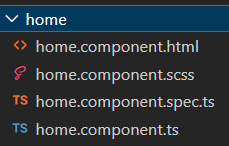
\includegraphics[scale=1]{images/componentStructure.PNG}
    \caption{Component Struktur [Quelle: Autor]}
\end{figure}
Um ein Component zu erstellen verwendet man in Angular folgenden Command:\\\
\begin{minted}[frame=single,framesep=0.2pt]{cpp}
ng generate component NameDerComponente
\end{minted}
Dieser Command kann auch abgekürzt werden, welcher dann folgendermaßen aussieht:\\\
\begin{minted}[frame=single,framesep=0.2pt]{cpp}
ng g c NameDerComponente
\end{minted}
In der Praxis ist es gängig, dass man alle Components in ein Unterverzeichnis namens 'components' speichert, so dass die gesamte Projektstruktur eine gewisse Ordnung behält. Nachdem ein Component erstellt wurde, kann diese in einem HTML File mithilfe des sogenannten Component Selector angezeigt werden. In der Abbilding 2.2 wurde ein Filter Component erstellt, dessen Selector als 'app-filter' bezeichnet wird. Um dieses Component aufzurufen deklariert man den Selector der Component im jeweiligen HTML File mit '<app-filter></app-filter>'.

\begin{figure}[H]
    \centering
    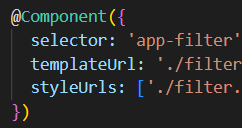
\includegraphics[scale=1]{images/selector.PNG}
    \caption{Component Selector [Quelle: Autor]}
\end{figure}

\subsection{Services}
Services oder auch als Serviceklassen bezeichnet, spielen eine bestimmte Rolle in Angular. Zu einem können sie als Schnittstelle zwischen Angular und dem Backend verwendet werden, zum anderen um die Kommunikation zwischen Components zu ermöglichen, wobei dieses Konzept später weiter erläutert wird.\\\
Components müssen häufig bestimmte Daten von einer Datenbank zum Beispiel anzeigen. Für dies muss zuerst ein HTTP Request an ein Backend geschickt werden, welches schlussendlich auf die Datenbank zugreift und die bestimmten Daten an das Frontend schickt. Services dienen hierbei als Schnittstelle zwischen Frontend und Backend. Sie kümmern sich in diesem Fall um das Abschicken und Empfangen von Requests und Responses. Dadurch ist eine klare Arbeitsaufteilung innerhalb der Projektstruktur von Angular möglich. Components kümmern sich um das Darstellen von Daten und Services, um diese Daten zum Beispiel von einem Backend Server abzurufen.\\\
Für das Erstellen von Services kann man die Angular cli verwenden. Ähnlich wie bei der Component Generierung, verwendet man für Services folgenden Command:
\begin{minted}[frame=single,framesep=0.2pt]{cpp}
ng generate services NameDesServices
\end{minted}
Hier ist es möglich den Command in gekürzter Form anzugeben:
\begin{minted}[frame=single,framesep=0.2pt]{cpp}
ng g s NameDesServices
\end{minted}
In der Praxis ist es üblich, Services in einem Unterverzeichnis namens 'services' zu speichern, damit eine klare Trennung zwischen Components und Services besteht. Für die Verwendung von Services kann ein Component dieses in sein Konstruktor innjecten. Dieses Konzept nennt man Dependency Injection. Dabei deklariert man im Konstruktur des Components den Service, der benutzt werden soll. Wenn eine Service als Injectable angegeben ist, kann diese in einem Component injeziert werden.

\subsection{Routing}
In einer Single Page Aplikation ändern man, was die Nutzende sehen, indem Teile der Webseite ein- oder ausgeblendet werden, die bestimmten Components entsprechen. In diesem Fall wird nicht der Server aufgerufen, um eine neue Seite zu erhalten. Wenn Nutzende Anwendungsaufgaben ausführen, müssen sie zwischen den verschiedenen Ansichten wechseln, die definiert wurden.
Für die Navigation von einer Ansicht zur nächsten, verwendet man den Angular Router. Der Router ermöglicht die Navigation, indem er eine Browser-URL als Anweisung zum Ändern der Ansicht interpretiert.\\\
Für die Verwendung des Angular Routers, muss dieser im 'app.module.ts' File importiert werden.\cite{angularrouter}
\begin{figure}[H]
    \centering
    
\includegraphics[scale=1]{images/importRouter.PNG}
    \caption{Importing Angular Router [Quelle: Autor]}
\end{figure}
\textbf{Definition der Routen}\\\
Damit zwischen einzelnen Routen gewechselt werden kann, ist es notwendig zunächst die Routen zu definieren. Dabei gibt man an welches Component bei einer bestimmten Route angezeigt wird. Man weist einen URL Pfad zu einem bestimmten Component. Abbildung 2.4 stellt ein Array von verschiedenen Routen dar. Das Array besteht aus Objekten, welches einen Pfad und ein Component beinhaltet. Im Pfad wird der Name von der Route beschrieben und beim Component, welches Component angezeigt werden soll, wenn auf diesen bestimmten Pfad navigiert. Navigiert man zum Beispiel zur '/home' URL, wird das Home Component geladen und angezeigt.\cite{angularrouter}
\begin{figure}[H]
    \centering
    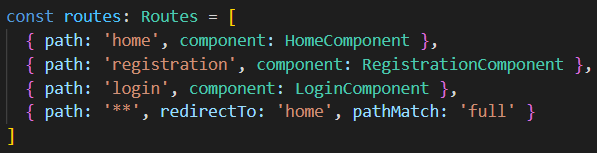
\includegraphics[scale=1]{images/routes.PNG}
    \caption{Route Definition [Quelle: Autor]}
\end{figure}
\textbf{Angular Router Konfiguration}\\\
Nachdem die einzelnen Routen erstellt wurden, muss der Router mit diesen konfiguriert werden. Dies geschieht mithilfe der 'RouterModule.forRoot()' Methode. Dieser Methode übergibt man das vorhin erstellte Array, die die Routen beinhaltet. Somit weiß der Angular Router über die einzelnen Routen bescheid und kann nach einer Navigation zu einem bestimmten Pfad, das entsprechende Component laden.\cite{angularrouter}

\begin{figure}[H]
    \centering
    
\includegraphics[scale=1]{images/routerModuleroot.PNG}
    \caption{Angular Router Konfiguration [Quelle: Autor]}
\end{figure}
\textbf{Route mit Parameterübergabe}\\\
Navigiert man zu einem bestimmten Pfad, kann ein Parameter mitgegeben werden. Dieser muss im vorhinein bei der Routen Definition angegeben. Der Parameter dient hierbei als Platzhalter. Zum Beispiel kann eine ID mitgegeben werden. Beim Laden des jeweiligen Components kann vom Pfad diese ID ausgelesen werden, um anschließend bestimmte Daten im Component anzeigen zu lassen, die dieser ID entsprechen. Oft ist hier der Fall, dass die ID vom Pfad ausgelesen wird und anschließend ein HTTP Request an ein Backend Server gesendet wird, um zu einer bestimmten Datei zusätzliche Informationen anzeigen zu lassen. In der Abbildung 2.6 ist eine Routen Definition mit einem Platzhalter namens 'ID' zu sehen, der das oben Beschriebene umsetzt.\cite{angularrouter}
\begin{figure}[H]
    \centering
    
\includegraphics[scale=1]{images/routeWithParam.PNG}
    \caption{Route Definition mit Parameter [Quelle: Autor]}
\end{figure}
Für das Zugreifen auf mitgegebene Parameter bei der Navigation, wird in Angular das ActivatedRouter Service injected. Mithilfe des Services kann man auf etwaige Properties von der Route Zugriff erhalten. Folgende Properties können bei der Navigation mitgegeben und anschließend abgerufen werden:
\begin{itemize}
    \item \textbf{url:} Ein Observable der Routenpfade, dargestellt als ein Array von Zeichenfolgen für jeden Teil des Routenpfads.
    \item \textbf{data:} 
Ein Observable, das das für die Route bereitgestellte Datenobjekt enthält. Enthält auch alle aufgelösten Werte aus dem Resolve Guard.
    \item \textbf{params:} Ein Observable, das die für die Route spezifischen erforderlichen und optionalen Parameter enthält.
    \item \textbf{paramMap:} Ein Observable, das eine Karte der für die Route spezifischen erforderlichen und optionalen Parameter enthält. Die Zuordnung unterstützt das Abrufen einzelner und mehrerer Werte aus demselben Parameter.
    \item \textbf{queryParamMap:} 
Ein Observable, das eine Karte der für alle Routen verfügbaren Abfrageparameter enthält. Die Zuordnung unterstützt das Abrufen einzelner und mehrerer Werte aus dem Abfrageparameter.
    \item \textbf{queryParams:} Ein Observable, das die für alle Routen verfügbaren Abfrageparameter enthält.
    \item \textbf{fragment:}
Ein Observable des URL-Fragments, das für alle Routen verfügbar ist.
    \item \textbf{outlet:} 
Der Name des RouterOutlet, das zum Rendern der Route verwendet wird. Bei einem unbenannten Ausgang ist der Name des Ausgangs primär.
    \item \textbf{routeConfig:}
Die Routenkonfiguration, die für die Route verwendet wird, die den Ursprungspfad enthält.
    \item \textbf{parent:} 
Die übergeordnete ActivatedRoute der Route, wenn diese Route eine untergeordnete Route ist.
    \item \textbf{firstChild:} Enthält die erste ActivatedRoute in der Liste der untergeordneten Routen dieser Route.
    \item \textbf{children:} 
Enthält alle unter der aktuellen Route aktivierten untergeordneten Routen.
\end{itemize}\cite{angularrouter}\\\
\textbf{Default Route}\\\
Die letzte Route Definition in der Abbildung 2.4 stellt einen Default Pfad dar. Navigiert man zu einem Pfad der nicht existiert bzw. vom Router nicht gefunden wird, so lädt der Router das Component welches unter dem Default Pfad angegeben ist. Wenn ein Nutzende die Webseite lädt, wird zu diesem Pfad weitergeleitet.
Bevor der Router zum Einsatz kommen kann, muss das sogenannte RouterOutlet Directive im HTML File angegeben werden. Typischerweise passiert dies im HTML File vom App Component. Hierbei definiert man das RouterOutlet directive als HTML Tag '<router-outlet></router-outlet>'. Dieses directive dient als Platzhalter, für die definierten Routen im Angular Router. Dort wo das RouterOutlet directive platziert wird, werden die Components angezeigt, wenn zu deren Pfade navigiert wird.\cite{angularrouter}\\\\\\
\textbf{Router Links}\\\
Für die Navigation an sich bietet Angular eine bestimmte Funktionalität namens Router Links an. Abbildung 2.7 1. Zeile, sieht man eine einfache Routing Navigation. Dem Anchor Tag wird ein Attribut namens 'routerLink' hinzugefügt. Diesem Attribut übergibt man einen Pfad, zu dieser der Angular Router navigiert, wenn auf den Anchor Tag geklickt wird.
\begin{figure}[H]
    \centering
    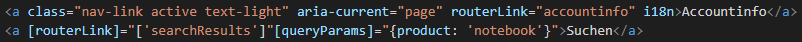
\includegraphics[scale=0.8]{images/routingNavigation.PNG}
    \caption{Router navigation [Quelle: Autor]}
\end{figure}
Müssen zusätzliche Properties oder Query Parameter dem Pfad beim Navigieren mitgegeben werden, kann dies mit '[routerLink]' durchgeführt werden. Durch die eckigen Klammern, wird dem Angular Router Bescheid gegeben, dass neben dem Pfad auch zusätzliche Informationen mitgegeben werden können. Hierbei könnte es sich um eine definierte Variable in einem Component File handeln, oder dynamische Werte. In Abbildung 2.7 2. Zeile, würde dieser Pfad folgende Route entsprechen, '/searchResults?product=notebook'. Mit [queryParams] teilt man den Angular Router mit, dass er neben dem Pfad zusätzlich den Query Parameter namens 'product', mit dem Wert 'notebook' übergeben soll.\cite{angularrouter}\\\\\\
\textbf{Activated Route}\\\
Befinden sich die Nutzende auf einer bestimmten Seite, kann das RouterLinkActive Directive benutzt werden, um CSS Klassen aktiv zu machen. Einem Anchor Tag kann man CSS Styles hinzufügen, so dass die Nutzende erkennen, auf welcher Seite sie sich gerade befinden und dies auch zum Beispiel im Menü ersichtlich markiert wird.
Damit ein Anchor Tag, nachdem zu einer bestimmten Seite navigiert wurde, CSS Styles erhält, fügt man dem Anchor Tag das RouterLinkActive Directive hinzu. Als Wert übergibt man eine oder mehrere CSS Klassen. In Abbildung 2.8 wird für den Anchor Tag die CSS Klasse 'activeSite' hinzugefügt, wenn die Anwendende zur Startseite navigieren.
\begin{figure}[H]
    \centering
    \includegraphics[scale=0.8]{images/routerLinkActive.PNG}
    \caption{Router navigation [Quelle: Autor]}
\end{figure}
Zusätzlich zu 'routerLinkActive' kann man auch '[routerLinkActive]' verwenden, um den Wert vom Directive auf ein Property des Components zu setzen.\cite{angularrouter}\\\

\textbf{Route Protection}\\\
Gewisse Routen sind für die Anwendende nicht zugänglich. Sei es eine Dashboard Seite nachdem man sich angemeldet hat oder eine Admin Seite. Bestimmte Routen sollen nicht für die Nutzende zugänglich sein. Daher ist es wichtig diese Routen zu schützen und nur Zugang zu gewährleisten, wenn sich Nutzende erfolgreich authentifizieren.
Für die Implementierung kommt das CanActivate Interface zum Einsatz. Dieses Interface wird in einer Guard Klasse verwendet. Durch das hinzufügen des CanActivate Interfaces, wird eine Methode namens canActivate in den Guard implementiert. Diese Methode bestimmt durch das Returnen von true oder false, ob eine Route zugänglich ist oder nicht. Dazu wird bei der Route Definition ein weiteres Property namens canActivate benutzt. Als Wert für das Property kann ein oder mehrere Guards verwendet werden. Returnen alle Guards true, können die Nutzende zu der geschützten Route navigieren. Wenn ein Guard false returned, ist die Route nicht zugänglich.
\begin{figure}[H]
    \centering
    \includegraphics[scale=0.8]{images/canActivate.PNG}
    \caption{CanActivate Methode [Quelle: Autor]}
\end{figure}
In Abbilding 2.9 wird ein Beispiel für die CanActivate Methode demonstriert. In diesem Beispiel lautet die Bedingung für das Zugreifen auf Routen, die mit diesem Guard gesichert sind, das die Anwendende angemeldet sein müssen. Ist dies der Fall, wird true returned, im anderen Fall wird auf die Default Route navigiert. Dieser Guard muss in der Route Definition im app.module.ts File eingefügt werden, indem der Wert des entsprechenden Propertys mit diesem gesetzt wird.
\begin{figure}[H]
    \centering
    \includegraphics[scale=0.8]{images/routeDefCanActivate.PNG}
    \caption{Guard in der Route Definition [Quelle: Autor]}
\end{figure}
\textbf{Child Routes}\\\
Child Routes oder auch Nested Routes genannt, sind Routen die nicht vom Root Component abgeleitet sind, sondern von einem anderen Component. Wenn die Web Applikation komplexer wird, macht es Sinn auf Child Routes zurückzugreifen. Denn bestimmte Seiten sind erst aufrufbar, wenn die Nutzende auf eine bestimmte Seite navigiert haben, von dieser eine andere Seite abgeleitet wird. Ein Beispiel dafür wäre eine Dashboard Seite. Von der Dashboard Seite kann man auf eine Account Information Seite navigieren. Würde man in der URL nur den Pfad von der Account Information Seite angeben, so wäre diese nicht aufrufbar, da man sich zuvor auf der Dashboard Seite befindet muss. Dadurch entsteht eine Baumstruktur von Routen, wobei Child Routen als Leaf Nodes agieren oder als Parent Node....

\subsection{Component Kommunikation}
\textbf{Parent-to-child Kommunikation}\\\
\textbf{Child-to-parent Kommunikation}\\\
\textbf{Kommunikation über Serviceclass}

\newpage
\section{Next.js}
\subsection{Routing}
\textbf{Wie funktioniert Routing}\\\
\textbf{Definition der Routen}\\\
\textbf{Navigation zwischen unterschiedliche Routen}\\\
\textbf{Route mit Parameterübergabe}\\\
\textbf{Route Protection}\\\

\subsection{Component Kommunikation}
\textbf{Parent-to-child Kommunikation}\\\
Properties\\\\\\
\textbf{Child-to-parent Kommunikation}\\\
Function properties\\\\\\
\textbf{Centralized State}

\newpage
\section{Unterschiede}
\subsection{Routing Unterscheidungen}
\subsection{Component-interaction Unterscheidungen}

\newpage
\chapter{Schluss}
\section{Zusammenfassung}
Wichtigsten Erkenntnisse noch einmal zusammenfassen
\section{Zukunfsausblicke}
Mögliche Themen die in zukünftigen Paper ausgearbeitet werden können

\newpage
\chapter{Related Work}


\newpage

% --- Bibliography ------------------------------------------------------

%IEEE Citation [1]:
\bibliographystyle{IEEEtran}
%for alphanumeric citation eg.: [ABC19]
%\bibliographystyle{alpha}

% List references I definitely want in the bibliography,
% regardless of whether or not I cite them in the thesis.

\newpage
\addcontentsline{toc}{chapter}{Bibliographie}
\bibliography{testBib}

\newpage

% --- List of Figures ----------------------------------------------------

\addcontentsline{toc}{chapter}{Abbildungen}
\listoffigures


% --- List of Tables -----------------------------------------------------

\newpage
\addcontentsline{toc}{chapter}{Tabellen}
\listoftables

% --- Appendix A -----------------------------------------------------

\newpage
\backmatter
\appendix
\begin{appendices}
\chapter{Appendix}

(Hier können Schaltpläne, Programme usw. eingefügt werden.)

\clearpage
\end{appendices}

\end{document}
